\documentclass{paper}

%\usepackage{times}
\usepackage{epsfig}
\usepackage{graphicx}
\usepackage{mathtools}
\usepackage{amssymb}
\usepackage{color}
\usepackage{caption}
\usepackage{subcaption}
\usepackage{natbib}

% load package with ``framed'' and ``numbered'' option.
%\usepackage[framed,numbered,autolinebreaks,useliterate]{mcode}

% something NOT relevant to the usage of the package.
\setlength{\parindent}{0pt}
\setlength{\parskip}{18pt}






\usepackage[latin1]{inputenc} 
\usepackage[T1]{fontenc} 

\usepackage{listings} 
\lstset{% 
   language=Matlab, 
   basicstyle=\small\ttfamily, 
} 



\title{Report for assignment 2}



\author{Moser Stefan\\09-277-013}
% //////////////////////////////////////////////////


\begin{document}



\maketitle

\section{Binocular Stereo (Due on 18/11/2013)}

In this assignment, we take a closer look at the
 the normalized 8-Point-Algorithm, as described by Richard Hartley \cite{601246}.

\subsection{Epipolar line estimation}

We let the user choose at least 8 corresponding points, then use this information to compute the fundamental matrix and draw epipolar lines.

\subsubsection{Normalizing points}

First, the user input is turned into homogeneous coordinates by appending a 1 to every point. 
In a further step, the centroid is removed from each point and the distance to the center normalized to two pixels. For this purpose, we construct a normalization matrix $M_p$ for the given points $p$, their centroid $c$ and their mean distance to the centroid $\overline{d}$ as:
\begin{equation}
M_p =
\begin{pmatrix}
	2/\overline{d} & 0 & -2/\overline{d} \cdot c_x \\
	0 & 2/\overline{d} & -2/\overline{d} \cdot c_y \\
	0 & 0 & 1
\end{pmatrix}
\end{equation}
So when multiplying it with an arbitrary point $(x,y,1)^T$ we get
\begin{equation}
M_p \begin{pmatrix}
 x \\
 y \\
 1
\end{pmatrix}
 = \begin{pmatrix}
 	\frac{2x}{\overline{d}} - \frac{2}{\overline{d}}c_x \\
 	\frac{2y}{\overline{d}} - \frac{2}{\overline{d}}c_y \\
 	1
 \end{pmatrix}
\end{equation}
which has exactly the desired effect described above.

\subsubsection{Computing Fundamental matrix}
For the given, normalized corresponding points from the base image (or left image in our case) $p$ and from the second (or right) image $p'$ 
we want to solve 
\begin{equation}
	p'^T F p = 0
\end{equation}
which is, as shown on the slides, the same as minimizing
\begin{equation}
	\sum_i ({p'}_i^T F p_i)^2
\end{equation}
under the constraint $||F||^2 = 1$. Minimizing this sum can be done using the SVD of a matrix $K$ with rows $i$ as
\begin{equation}
K_i = 
\begin{pmatrix}
 u_i'u_i & u_i'v_i & u_i' & v_i'u_i & v_i'v_i & v_i' & u_i & v_i & 1 
\end{pmatrix}
\end{equation}
with $p_i = (u_i,v_i,1)$, $p_i' = (u_i',v_i',1)$ for every pair of corresponding points $i$. When we now compute the SVD
\begin{equation}
	[U_K, D_K, V_K] = \text{svd}(K)
\end{equation}
From the construction of the SVD we know, that the column of $V_K$ corresponding to the minimal eigenvalue (ie. the last) does meet all
requirements mentioned above. So it corresponds to our normalized
fundamental matrix $\hat{F}_{r3}$. To ensure rank 2 we use again SVD, 
discard the third (and smallest) eigenvalue and reconstruct $\hat{F}_{r2}$. 
To obtain our final fundamental matrix $F$, we remove the normalization introduced in the previous section by computing 
   \begin{equation}
   F = M_{p'}^ T \hat{F}_{r2} M_p
   \end{equation}
   
\subsubsection{Drawing epipolar lines}
To draw the epipolar line $e$ corresponding to the point $p$ on the base image, we simply compute
\begin{equation}
	e = F p
\end{equation}
$e$ can then be used to extrapolate image coordinates, through which a line then can be matched. 
To cover every edge case, I extrapolated four points: $x_0 = 0, y_1 = 0, x_2 = w, y_3 = h$ (with $h$ as image height and $w$ as width). 
In the same way, the epipolar line for a given point $p'$ on the secondary image can be computed as
\begin{equation}
	e' = F^Tp'
\end{equation} 
\begin{figure}
\centering
\begin{subfigure}{0.49\textwidth}
   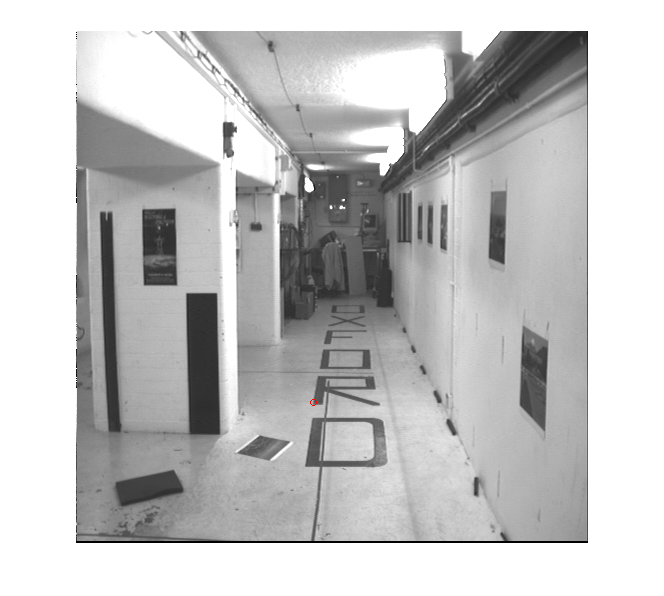
\includegraphics[width=\textwidth]{corridor_epipolar_line}
   \caption{Point chosen on left image}
   \label{fig:corridor_point}
\end{subfigure}
\begin{subfigure}{0.49\textwidth}
   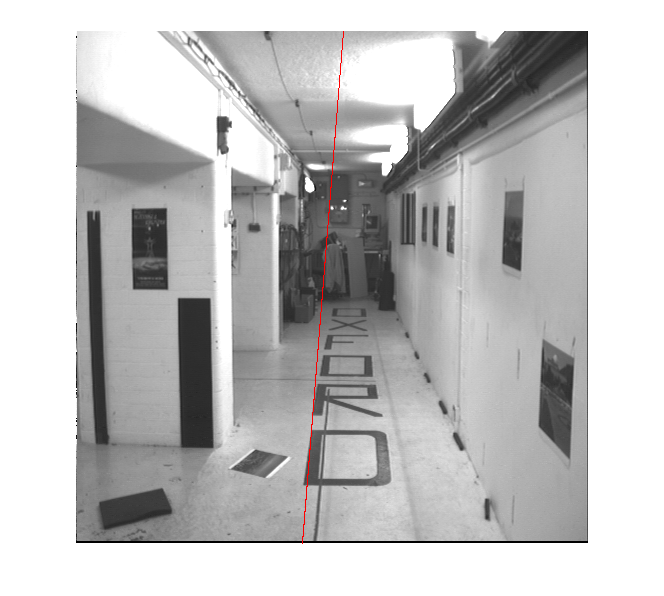
\includegraphics[width=\textwidth]{corridor_epipolar_line_r}
   \caption{Epipolar line on right image}
\end{subfigure}
\begin{subfigure}{0.49\textwidth}
   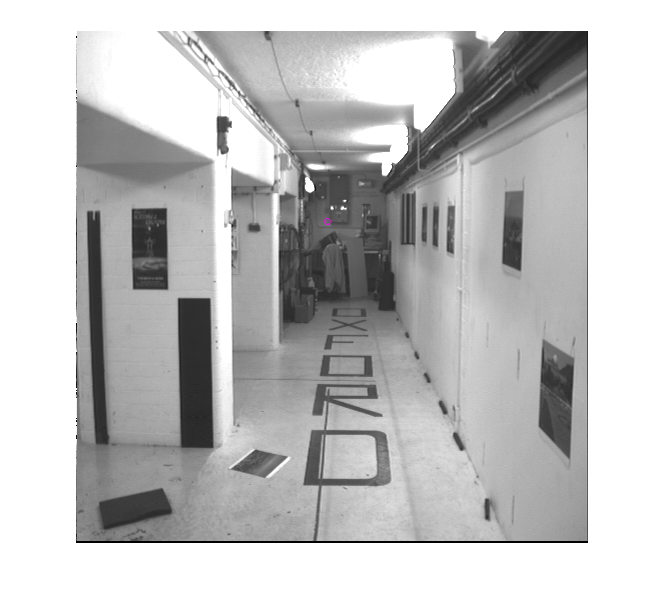
\includegraphics[width=\textwidth]{corridor_epipole}
   \caption{Epipole}
\end{subfigure}
\caption{The estimation of an epipolar line and epipole 
on the corridor scene. 
For the estimation of the fundamental matrix, 9 points were given.}
\label{fig:corridor}
\end{figure}

\subsubsection{Computing the epipoles}
We know that the epipoles lie in the null space of $F$ respectively $F'$. For
obtaining them, we can simply use the matlab function \emph{null} and scale 
the result to image coordinates by scaling it in such a way that 
the z-coordinate is one.
 
\subsection{Model reconstruction}
This time, the corresponding points are not given as user input, but
read out from a file. We take an arbitrary large subset of them 
(larger than 8) to compute the fundamental
matrix and further the essential matrix. Then we estimate the depth of these points.

\subsubsection{Computing the essential matrix}
We retrieve the fundamental matrix $F$ as described in the section before. To
retrieve the essential matrix, we need to use the cameras intrinsic parameters $K$ respectively $K'$ for the secondary view:
\begin{align}
	 F &= K'^{-T} E K^{-1} \\
	\Longleftrightarrow E &= K'^T F K
\end{align}
For our computation, we had $K = K'$ given. 
\subsubsection{Estimate the rotation and translation}

From the slides we know that the essential matrix consists of a translation $T_\times$ (expressed as skew symmetric matrix) and a rotation $R$:
\begin{equation}
	E = T_\times R
\end{equation}
To split E into these two parts, we can use the SVD of $E$, which gives us
\begin{equation}
	E = UDV^T
\end{equation}
If we define now
\begin{equation}
 W = \begin{pmatrix}
 	0 & -1 & 0 \\
 	1 & 0 & 0 \\
 	0 & 0 & 1
 \end{pmatrix}
\end{equation}
we can easily derive the translation
\begin{equation}
T_\times = V W D V^T
\end{equation}
and the rotation
\begin{equation}
R = U W^{-1} V^T
\end{equation}

\subsubsection{Obtaining depth}
This algorithm has been first described by Longuet-Higgins \cite{Longuet-Higgins87}. For brevity, we just summarize the most important equations. For
a point $p$ on the base image and its corresponding point $p'$, we can compute the corresponding 3D point $P$ as
\begin{equation}
 P_3 = \frac{(R_1 - p'_1 R_3) \cdot T}{(R_1 - p'_1 R_3) \cdot p}
\end{equation}
with $T$ as translation vector and $R_i$ the $i$'th row of the rotation matrix $R$. The other coordinates of $P$ can then be computed as
\begin{equation}
 P = (p_1 \cdot P_3, p_2 \cdot P_3, P_3)
\end{equation}
\begin{figure}
\centering
\begin{subfigure}{0.3\textwidth}
   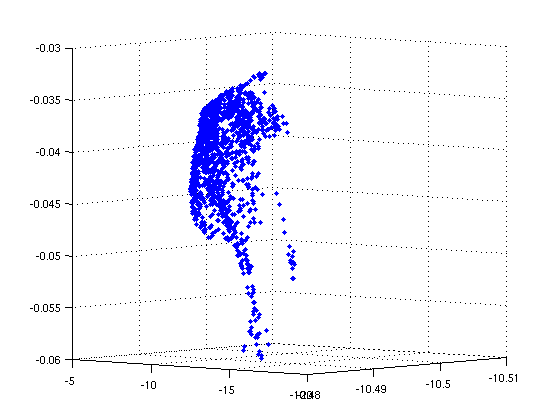
\includegraphics[width=\textwidth]{cow_depths}
\end{subfigure}
\begin{subfigure}{0.3\textwidth}
   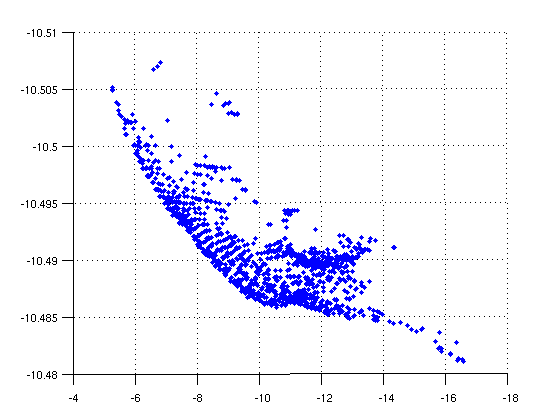
\includegraphics[width=\textwidth]{cow_depths_above}
\end{subfigure}
\begin{subfigure}{0.3\textwidth}
   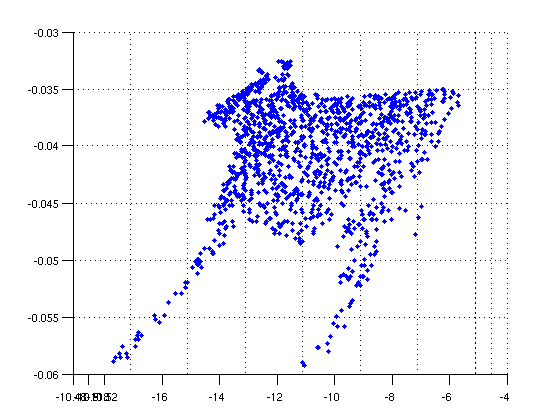
\includegraphics[width=\textwidth]{cow_depths_side}
\end{subfigure}
\caption{The cows depth reconstructed using 10 percent of the points given.
The essential matrix was not reconstructed, but computed using the ground
truths rotation and translation.}
\label{fig:cow}
\end{figure}
The results obtained are visible in figure \ref{fig:cow}.
\subsection{Discussion}
While this algorithm is very simple and easy to implement, it is also very sensitive
to noise. If we added some noise to the correspondences, the results from figure \ref{fig:corridor} would look completely different, 
which can be seen in figure \ref{fig:corridor_noisy}.
\begin{figure}[h]
\centering
   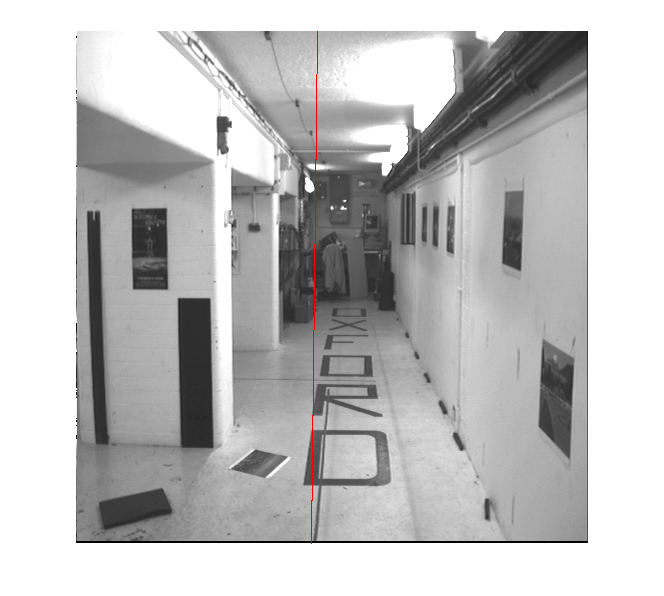
\includegraphics[width=\textwidth]{corridor_eline_noisy}
\caption{The points chosen on the left image had some gaussian noise 
($\mu = 0, \sigma = 3$) added. The epipole drawn is for
the same point as shown in figure 
\ref{fig:corridor_point},
 but the result is completely off, with the epipole not even
on the image anymore.}
\label{fig:corridor_noisy}
\end{figure}
 There are plentiful other ways for estimating the fundamental matrix, eg.
\begin{itemize}
\item 8-Point unnormalized
\item Iteratively minimizing the geometric error \cite{Hartley2004}, with various norms
\item Iteratively minimizing the algebraic error \cite{Hartley2004}, with various norms
\end{itemize}
It is a widely accepted fact that the unnormalized 8-point algorithm performs much worse
than any other due to numerical instability. 
Other iterative algorithms perform better in the presence of noise. They 
also, as with any other iterative algorithm, make it easier to handle large amounts of matched points: When a
desired bound is reached, the algorithm can just stop and 
return the current result. The 8-point algorithm has to
solve the whole linear system before it can produce a result.
    Omid Aghazadeh is offering some code online
\footnote{http://www.mathworks.ch/matlabcentral/fileexchange/27541-fundamental-matrix-computation}  that can be used to 
compare the performance of the algorithms mentioned under various noise conditions. Figure \ref{fig:comparison} 
was compiled using his code.
\begin{figure}
\centering
\begin{subfigure}{0.4\textwidth}
   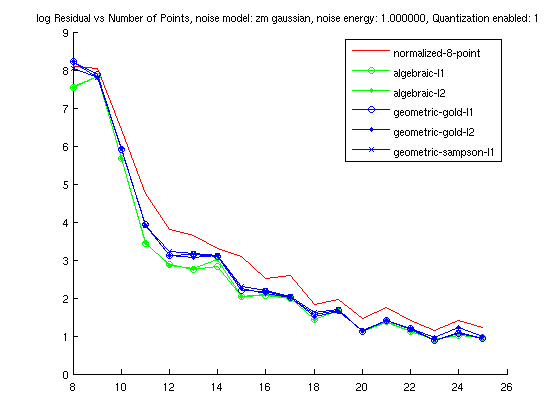
\includegraphics[width=\textwidth]{noise_norm1}
   \caption{Gaussian noise, energy 1}
\end{subfigure}
\begin{subfigure}{0.4\textwidth}
   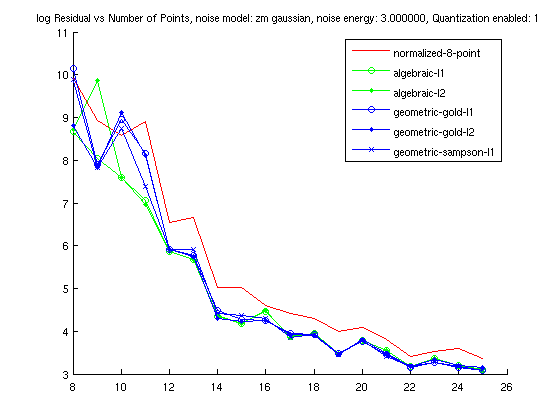
\includegraphics[width=\textwidth]{noise_norm3}
   \caption{Gaussian noise, energy 3}
\end{subfigure}
\begin{subfigure}{0.4\textwidth}
   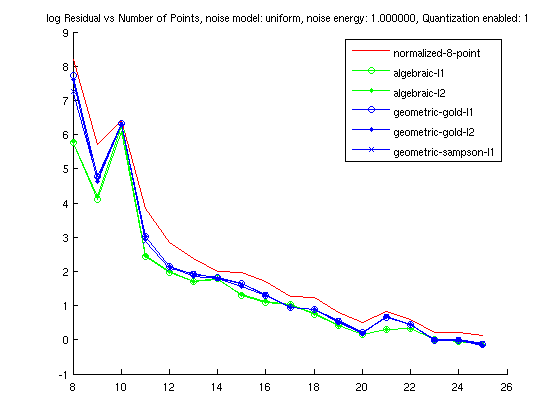
\includegraphics[width=\textwidth]{noise_uniform1}
   \caption{Uniform noise, energy 1}
\end{subfigure}
\begin{subfigure}{0.4\textwidth}
   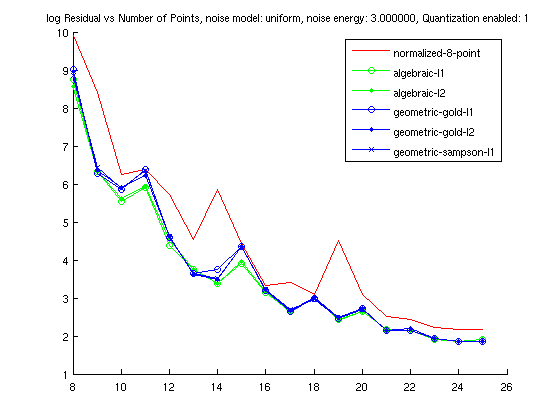
\includegraphics[width=\textwidth]{noise_uniform3}
   \caption{Uniform noise, energy 3}
\end{subfigure}
\caption{Comparison of various different algorithms for computing the 
fundamental matrix. Especially with higher noise energy, the normalized 8-point
algorithm falls behind in performance for almost any amount of points given.}
\label{fig:comparison}
\end{figure}
\bibliographystyle{plain}
\bibliography{Report_2_Stefan_Moser}
\end{document}